
%
%	Measurement of NCQE cross section in SK-Gd
%

\section{Measurement of NCQE cross section in SK-Gd}\label{Sec_NCQE}
\Headerfooter{Measurement of NCQE cross section in SK-Gd}





\subsection{Measured NCQE cross section}
\vs\hs
The atmospheric neutrino flux-averaged theoretical neutrino-oxygen NCQE cross section is
\begin{eqnarray}
	\langle \sigma^{\rm theory}_{\rm NCQE} \rangle &=& \frac{\int_{\rm 160\,MeV}^{\rm 10\,GeV}\sum_{i=\nu,\bar{\nu}}\phi_{i}(E)\times\sigma_{i}(E)^{\rm theory}_{\rm NCQE}dE}{\int_{\rm 160\,MeV}^{\rm 10\,GeV}\sum_{i=\nu,\bar{\nu}}\phi_{i}(E)dE} \nonumber \\
																								 &=& 1.02 \times 10^{-38}\,{\rm cm}^{2}/{\rm oxygen},\label{Eq_theory}
\end{eqnarray}
where $\phi_{i}(E)$ is the atmospheric neutrino flux~\cite{2011Honda} at neutrino energy $E$ and $\sigma_{i}(E)^{\rm theory}_{\rm NCQE}$ is the theoretical NCQE cross section~\cite{2012Ankowski}.
The integral is performed between 160~MeV and 10~GeV because the NCQE cross section is small below 160~MeV and the atmospheric neutrino flux is small above 10~GeV (see Figure~\ref{Simula_AtmNeuFlux} and Figure~\ref{Simula_NCQECroSec}).
The systematic uncertainty by the energy cutoff is described in Section~\ref{SYSTEM}.
The measured neutrino-oxygen NCQE cross section is
\begin{eqnarray}
	\langle \sigma^{\rm measured}_{\rm NCQE} \rangle &=&\frac{N^{\rm obs}-N^{\rm exp}_{\rm Non\mathchar`-NCQE}}{N^{\rm exp}_{\rm NCQE}}\times\langle \sigma^{\rm theory}_{\rm NCQE} \rangle \nonumber \\
																									 &=& 0.74 \pm 0.22 ({\rm stat.}) \times 10^{-38}\,{\rm cm}^{2}/{\rm oxygen},\label{Eq_measured}
\end{eqnarray}
where $N^{\rm obs}$~($=38$) is the observed number of events, $N^{\rm exp}_{\rm NCQE}$~($=28.7071$) is the expected number of NCQE events, and $N^{\rm exp}_{\rm Non\mathchar`-NCQE}$~($=17.1920$) is the expected number of non-NCQE events, including NC non-QE, CC, spallation, reactor neutrino, and accidental coincidence.
Here, the calculation of statistical uncertainty in Equation~(\ref{Eq_measured}) is described.
The fraction in Equation~(\ref{Eq_measured}) is redefined as
\begin{eqnarray}
	f_{\rm NCQE} = \frac{N^{\rm obs}-N^{\rm exp}_{\rm Non\mathchar`-NCQE}}{N^{\rm exp}_{\rm NCQE}}.\label{Eq_f_NCQE}
\end{eqnarray}
The statistical uncertainty of numerator $\delta N^{\rm numerator}$ is
\begin{eqnarray}
	\delta N^{\rm numerator} &=& \sqrt{(\delta N^{\rm obs})^{2} + (\delta N^{\rm exp}_{\rm Non\mathchar`-NCQE})^{2}} \nonumber \\
													 &=& \delta N^{\rm obs} \nonumber \\
													 &=& \sqrt{N^{\rm obs}}.
\end{eqnarray}
While the statistical uncertainty of denominator $\delta N^{\rm denominator}$ is
\begin{eqnarray}
	\delta N^{\rm denominator} &=& \delta N^{\rm exp}_{\rm NCQE} \nonumber \\
														 &=& 0.
\end{eqnarray}
Therefore, the statistical uncertainty of $f_{\rm NCQE}$ is
\begin{eqnarray}
	\delta f_{\rm NCQE} &=& |f_{\rm NCQE}| \times \sqrt{\bigg({\delta N^{\rm numerator} \over  N^{\rm numerator}}\bigg)^{2} + \bigg({\delta N^{\rm denominator} \over N^{\rm denominator}}\bigg)^{2}} \nonumber \\
											&=& |f_{\rm NCQE}| \times {\sqrt{N^{\rm obs}} \over N^{\rm obs}-N^{\rm exp}_{\rm Non\mathchar`-NCQE}} \nonumber \\
											&=& {\sqrt{N^{\rm obs}} \over N^{\rm exp}_{\rm NCQE}},
\end{eqnarray}
and the statistical uncertainty of $\langle \sigma^{\rm measured}_{\rm NCQE} \rangle$ is 
\begin{eqnarray}
	\delta \langle \sigma^{\rm measured}_{\rm NCQE} \rangle &=& \delta f_{\rm NCQE} \times \langle \sigma^{\rm theory}_{\rm NCQE} \rangle \nonumber \\
																													&=& 0.22 \times 10^{-38}\,{\rm cm}^{2}/{\rm oxygen}.
\end{eqnarray}





\subsection{Systematic uncertainties of the expected events}\label{SYSTEM}
\vs\hs
Systematic uncertainties of the expected NCQE, NC non-QE, and CC events are summarized in Table~\ref{tab:sys}.
We follow the estimation methods of measurements in SK pure water phase and T2K~\cite{2019Linyan,2014Abe,2019Abe}.
The estimation of each systematic uncertainty is described below.\\

\begin{table}[h]
	\centering
	\caption[Systematic uncertainties of the expected NCQE, NC non-QE, and CC events]{
	Systematic uncertainties of the expected NCQE, NC non-QE, and CC events.
	}\label{tab:sys}
	\vs
	\begin{tabular}{lrrr} \hline \hline
		                                        & NCQE                 & NC non-QE            & CC                   \\ \hline
		Atmospheric neutrino flux               & $\pm$18.0\%          & $\pm$18.0\%          & $\pm$18.0\%          \\
		Atmospheric neutrino/antineutrino ratio & $\pm$5.0\%           & $\pm$5.0\%           & $\pm$5.0\%           \\
		Cross section                           & -                    & $\pm$18.0\%          & $\pm$24.0\%          \\
		Primary interaction                     & $+$1.5\% / $-$9.4\%  & $+$0.0\% / $-$2.4\%  & $+$1.2\% / $-$8.0\%  \\
		Secondary interaction                   & $+$0.0\% / $-$30.9\% & $+$0.0\% / $-$24.3\% & $+$0.0\% / $-$20.7\% \\
		Energy cutoff                           & $+$0.0\% / $-$2.1\%  & $+$0.0\% / $-$1.5\%  & $+$0.0\% / $-$19.9\% \\
		Data reduction                          & $\pm$1.4\%           & $\pm$1.4\%           & $\pm$1.4\%           \\
		Neutron tagging                         & $\pm$6.4\%           & $\pm$6.4\%           & $\pm$6.4\%           \\ \hline \hline
	\end{tabular}
\end{table}

\textbf{Atmospheric neutrino flux}\\
\hs
The uncertainty of the measured atmospheric neutrino flux in SK differs in each energy bin, as shown in Table~\ref{tab:Flux} and Figure~\ref{Flux_error}~\cite{2016Richard}.
From Table~\ref{tab:Flux}, atmospheric neutrino flux uncertainty $\Delta{\rm \Phi}^{\nu}/{\rm \Phi}^{\nu}$ is calculated by considering the weight of flux in each energy bin, as
\begin{eqnarray}
	{\Delta{\rm \Phi}^{\nu} \over {\rm \Phi}^{\nu}} &=& \sum_{i=1}^{9} \Bigg({\Delta{\rm \Phi}_{i}^{\nu} \over {\rm \Phi}_{i}^{\nu}} \times {{\rm \Phi}_{i}^{\nu} \over \sum_{j=1}^{9} {\rm \Phi}_{j}^{\nu} + \sum_{j=12}^{19} {\rm \Phi}_{j}^{\nu}}\Bigg) \nonumber \\
																									& & + \sum_{i=12}^{19} \Bigg({\Delta{\rm \Phi}_{i}^{\nu} \over {\rm \Phi}_{i}^{\nu}} \times {{\rm \Phi}_{i}^{\nu} \over \sum_{j=1}^{9} {\rm \Phi}_{j}^{\nu} + \sum_{j=12}^{19} {\rm \Phi}_{j}^{\nu}}\Bigg) \nonumber \\
																									&=& 17.9\%.
\end{eqnarray}
In this measurement, we chose the conservative value and 18.0\% in [160~MeV, 10~GeV] is applied to atmospheric neutrino flux uncertainty.\\

\textbf{Atmospheric neutrino/antineutrino ratio}\\
\hs
Figure~\ref{Flux_ratio} shows the ratio of atmospheric neutrino flux~\cite{2007Honda}.
In the neutrino energy region below 10~GeV, the difference of atmospheric neutrino/antineutrino ratio due to the hadronic interaction models is less than 5.0\%.
Therefore, atmospheric neutrino/antineutrino ratio uncertainty is taken as 5.0\%.\\

\begin{table}[p]
	\centering
	\caption[Measured atmospheric neutrino flux using SK-I to SK-IV data]{
	Measured atmospheric neutrino flux using SK-I to SK-IV data~\cite{2016Richard}.
	Uncertainties are summarized in the rightmost column.
	}\label{tab:Flux}
	\vs
	\begin{tabular}{ccccc} \hline \hline
		$i$ & ${\rm log}_{10}$ & ${\rm log}_{10}$ & $\bar{E}_{i}^{2}{\rm \Phi}_{i}^{\nu}$ & $\Delta{\rm \Phi}_{i}^{\nu}/{\rm \Phi}_{i}^{\nu}$ \\
		                & $(E/{\rm GeV})$  & $(\bar{E}_{i}/{\rm GeV})$ & $({\rm GeV}/{\rm cm}^{2}/{\rm sec}/{\rm sr})$ & $(\%)$  \\ \hline
		$\nu_{{\rm e}}$ &                  &                           &                                               &         \\
		1               & $-$0.8 to $-$0.6 & $-$0.71                   & 1.21 $\times$ 10$^{-\text{2}}$                & $\pm$18 \\
		2               & $-$0.6 to $-$0.4 & $-$0.51                   & 1.46 $\times$ 10$^{-\text{2}}$                & $\pm$17 \\
		3               & $-$0.4 to $-$0.2 & $-$0.27                   & 1.50 $\times$ 10$^{-\text{2}}$                & $\pm$16 \\
		4               & $-$0.2 to 0.0    & $-$0.09                   & 1.37 $\times$ 10$^{-\text{2}}$                & $\pm$15 \\
		5               & 0.0 to 0.2       & 0.10                      & 1.16 $\times$ 10$^{-\text{2}}$                & $\pm$17 \\
		6               & 0.2 to 0.4       & 0.30                      & 8.55 $\times$ 10$^{-\text{3}}$                & $\pm$17 \\
		7               & 0.4 to 0.6       & 0.50                      & 6.09 $\times$ 10$^{-\text{3}}$                & $\pm$18 \\
		8               & 0.6 to 0.8       & 0.70                      & 3.73 $\times$ 10$^{-\text{3}}$                & $\pm$19 \\
		9               & 0.8 to 1.0       & 0.90                      & 2.32 $\times$ 10$^{-\text{3}}$                & $\pm$18 \\
		10              & 1.0 to 1.5       & 1.22                      & 9.42 $\times$ 10$^{-\text{4}}$                & $\pm$15 \\
		11              & 1.5 to 2.0       & 1.72                      & 2.03 $\times$ 10$^{-\text{4}}$                & $\pm$18 \\
		$\nu_{\mu}$     &                  &                           &                                               &         \\
		12              & $-$0.6 to $-$0.4 & $-$0.51                   & 1.58 $\times$ 10$^{-\text{2}}$                & $\pm$21 \\
		13              & $-$0.4 to $-$0.2 & $-$0.32                   & 1.77 $\times$ 10$^{-\text{2}}$                & $\pm$16 \\
		14              & $-$0.2 to 0.0    & $-$0.09                   & 1.86 $\times$ 10$^{-\text{2}}$                & $\pm$15 \\
		15              & 0.0 to 0.2       & 0.10                      & 1.68 $\times$ 10$^{-\text{2}}$                & $\pm$16 \\
		16              & 0.2 to 0.4       & 0.30                      & 1.38 $\times$ 10$^{-\text{2}}$                & $\pm$18 \\
		17              & 0.4 to 0.6       & 0.51                      & 9.59 $\times$ 10$^{-\text{3}}$                & $\pm$19 \\
		18              & 0.6 to 0.8       & 0.71                      & 6.68 $\times$ 10$^{-\text{3}}$                & $\pm$19 \\
		19              & 0.8 to 1.0       & 0.90                      & 4.79 $\times$ 10$^{-\text{3}}$                & $\pm$17 \\
		20              & 1.0 to 1.5       & 1.21                      & 2.62 $\times$ 10$^{-\text{3}}$                & $\pm$13 \\
		21              & 1.5 to 2.0       & 1.73                      & 1.20 $\times$ 10$^{-\text{3}}$                & $\pm$16 \\
		22              & 2.0 to 3.0       & 2.40                      & 2.49 $\times$ 10$^{-\text{4}}$                & $\pm$18 \\
		23              & 3.0 to 4.0       & 3.39                      & 1.46 $\times$ 10$^{-\text{5}}$                & $\pm$21 \\ \hline \hline
	\end{tabular}
\end{table}

\begin{figure}[p]
	\centering
	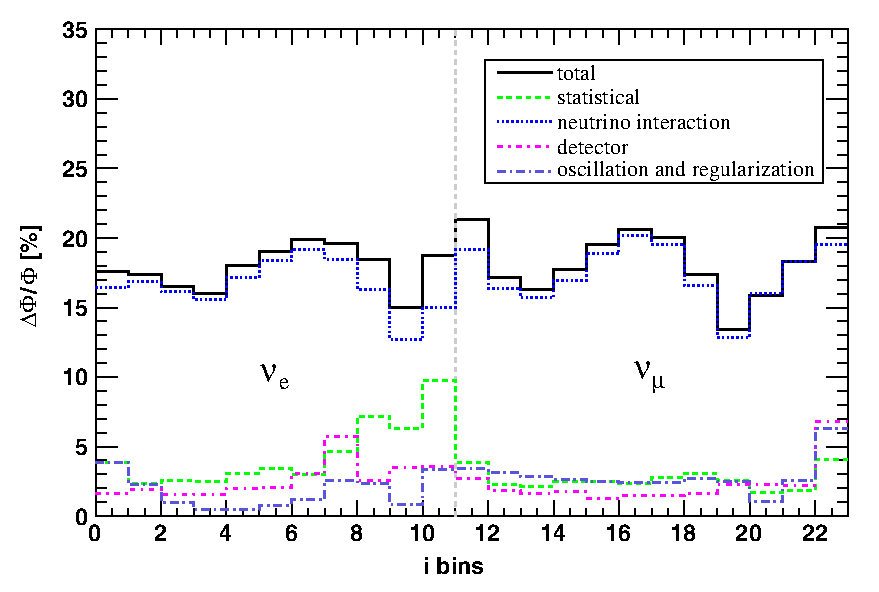
\includegraphics[width=10cm]{Figures/NCQE/Flux_error}
	\caption[Uncertainty of the measured atmospheric neutrino flux in SK]{
	Uncertainty of the measured atmospheric neutrino flux in SK~\cite{2016Richard}.
	Energy region of each bin is summarized in Table~\ref{tab:Flux}.
	Total uncertainty consists of statistical, neutrino interaction, detector response, and neutrino oscillation and regularization uncertainties.
	Details of these components are summarized in Ref.~\cite{2016Richard}.
	}\label{Flux_error}
\end{figure}

\begin{figure}[p]
	\centering
	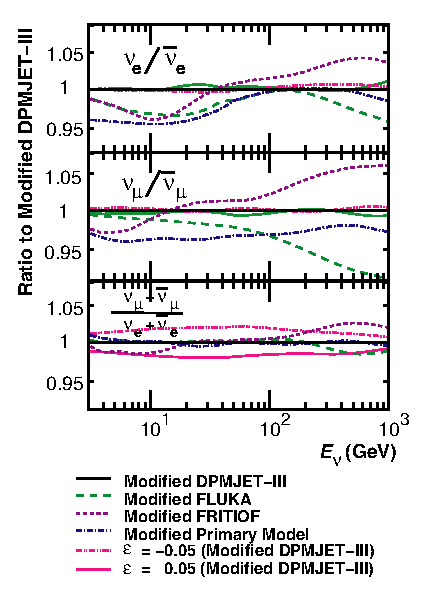
\includegraphics[width=8cm]{Figures/NCQE/Flux_ratio}
	\caption[Ratio of atmospheric neutrino flux]{
	Ratio of atmospheric neutrino flux~\cite{2007Honda}.
	}\label{Flux_ratio}
\end{figure}

\textbf{Cross section}\\
\hs
Cross section uncertainty is taken as 18.0\% for NC non-QE events and 24.0\% for CC events considering the uncertainties of parameters for the cross-section models such as the axial mass, normalization parameters for each interaction, and the decay width of resonant pion production~\cite{2014Abe,2015HuangPhD}.
Since the purpose of this study is to measure the NCQE cross section, the cross section uncertainty is not assigned for NCQE events.
Details of these cross section uncertainties are summarized in Section~6.1 of Ref.~\cite{2015HuangPhD}.\\

\textbf{Primary interaction}\\
\hs
Primary interaction uncertainty arises from the spectroscopic strengths of the oxygen nucleus.
Computation of the $p_{3/2}$ spectroscopic strength is consistent with $^{16}{\rm O}({\rm e}, {\rm e}^{\prime}{\rm p})$ experiment within 5.4\%~\cite{2012Ankowski,1994Leuschner}.
Therefore, the uncertainty of $(p_{3/2})^{-1}$ state is estimated by increasing the production probabilities of this state by 5.4\%.
For the \textit{others} state, there is no reliable predictions as written in Section~\ref{Subsec_neutrino_int}, thus the uncertainty is conservatively estimated by comparing with an extreme case, that is the difference between the default state ($(s_{1/2})^{-1}$) and the ground state ($(p_{1/2})^{-1}$).
The uncertainty is taken to be the difference in the expected number of events from the default condition to other conditions.
Table~\ref{tab:Pri} shows the production probabilities of $(p_{1/2})^{-1}$, $(p_{3/2})^{-1}$, and $(s_{1/2})^{-1}$ state and the expected number of NCQE, NC non-QE, and CC events in each condition of the primary interaction uncertainty estimation.
From this result, the primary interaction uncertainty is taken as $+$1.5\% / $-$9.4\%, $+$0.0\% / $-$2.4\%, and $+$1.2\% / $-$8.0\% for $N^{\rm exp}_{\rm NCQE}$, $N^{\rm exp}_{\rm NC\,non\mathchar`-QE}$, and $N^{\rm exp}_{\rm CC}$, respectively.\\
%Differences of the number and energy of gamma-rays and neutrons by each condition are shown from Figure~\ref{Comp_gammaNumPri} to Figure~\ref{Comp_neutronLogEnePri}.

\begin{table}[h]
	\centering
	\caption[Production probabilities of $(p_{1/2})^{-1}$, $(p_{3/2})^{-1}$, and $(s_{1/2})^{-1}$ state and the expected number of NCQE, NC non-QE, and CC events in each condition of the primary interaction uncertainty estimation]{
	Production probabilities of $(p_{1/2})^{-1}$, $(p_{3/2})^{-1}$, and $(s_{1/2})^{-1}$ state and the expected number of NCQE, NC non-QE, and CC events in each condition of the primary interaction uncertainty estimation.
	Differences of the expected number of events from the default condition are summarized in parentheses.
	}\label{tab:Pri}
	\vs
	\begin{tabular}{cccc} \hline \hline
		                               & \textit{others} $\to$ $(s_{1/2})^{-1}$ & \textit{others} $\to$ $(p_{1/2})^{-1}$ & $(p_{3/2})^{-1}$ $\times\,1.054$  \\
		                               & (Default)                              &                                        &                                   \\ \hline
		$(p_{1/2})^{-1}$               & 0.1580                                 & 0.5430                                 & 0.1390                            \\
		$(p_{3/2})^{-1}$               & 0.3515                                 & 0.3515                                 & 0.3705                            \\
		$(s_{1/2})^{-1}$               & 0.4905                                 & 0.1055                                 & 0.4905                            \\ \hline
		$N^{\rm exp}_{\rm NCQE}$       & 28.7071                                & 26.0172 ($-$9.4\%)                     & 29.1364 ($+$1.5\%)                \\
		$N^{\rm exp}_{\rm NC\,non-QE}$ & 13.2721                                & 12.9705 ($-$2.3\%)                     & 12.9520 ($-$2.4\%)                \\
		$N^{\rm exp}_{\rm CC}$         & 1.4177                                 & 1.3042 ($-$8.0\%)                      & 1.4346 ($+$1.2\%)                 \\ \hline \hline
	\end{tabular}
\end{table}

\textbf{Secondary interaction}\\
\hs
As described in Section~\ref{Subsec_Comp_data}, the chi-square differences were inconclusive.
Therefore, the secondary interaction uncertainty is taken to be the difference in the expected number of events from BERT to BIC or INCL++.
The expected number of NCQE, NC non-QE, and CC events in each condition of the secondary interaction uncertainty estimation is summarized in Table~\ref{tab:Sec}.
From this result, the secondary interaction uncertainty is taken as $-$30.9\%, $-$24.3\%, and $-$20.7\% for $N^{\rm exp}_{\rm NCQE}$, $N^{\rm exp}_{\rm NC\,non\mathchar`-QE}$, and $N^{\rm exp}_{\rm CC}$, respectively.\\

\begin{table}[tbp]
	\centering
	\caption[The expected number of NCQE, NC non-QE, and CC events in each condition of the secondary interaction uncertainty estimation]{
	The expected number of NCQE, NC non-QE, and CC events in each condition of the secondary interaction uncertainty estimation.
	Differences of the expected number of events from the default condition are summarized in parentheses.
	}\label{tab:Sec}
	\vs
	\begin{tabular}{cccc} \hline \hline
		                                         & BERT      & BIC                 & INCL++              \\
		                                         & (Default) &                     &                     \\ \hline
		$N^{\rm exp}_{\rm NCQE}$                 & 28.7071   & 19.8420 ($-$30.9\%) & 20.2027 ($-$29.6\%) \\
		$N^{\rm exp}_{\rm NC\,non\mathchar`-QE}$ & 13.2721   & 10.1887 ($-$23.2\%) & 10.0517 ($-$24.3\%) \\
		$N^{\rm exp}_{\rm CC}$                   & 1.4177    & 1.1244 ($-$20.7\%)  & 1.2173 ($-$14.1\%)  \\ \hline \hline
	\end{tabular}
\end{table}

\textbf{Energy cutoff}\\
\hs
In Equation~(\ref{Eq_theory}), the integral is performed between 160~MeV and 10~GeV, while the expected number of atmospheric neutrino events is estimated using full energy range.
Energy cutoff uncertainty is estimated considering the difference of these energy range.
Table~\ref{tab:Cutoff} shows the expected number of NCQE, NC non-QE, and CC events in each condition of the energy cutoff uncertainty estimation.
Since the expected number of events decreases by the energy cutoff, only a negative direction is considered, and the energy cutoff uncertainty is taken as $-$2.1\%, $-$1.5\%, and $-$19.9\% for $N^{\rm exp}_{\rm NCQE}$, $N^{\rm exp}_{\rm NC\,non\mathchar`-QE}$, and $N^{\rm exp}_{\rm CC}$, respectively.\\

\begin{table}[h]
	\centering
	\caption[The expected number of NCQE, NC non-QE, and CC events in each condition of the energy cutoff uncertainty estimation]{
	The expected number of NCQE, NC non-QE, and CC events in each condition of the energy cutoff uncertainty estimation.
	$E$ shows the neutrino energy.
	Differences of the expected number of events from the default condition are summarized in parentheses.
	}\label{tab:Cutoff}
	\vs
	\begin{tabular}{ccc} \hline \hline
		                                         & Full energy range & $E\in [160\,{\rm MeV}, 10\,{\rm GeV}]$ \\
		                                         & (Default)         &                                        \\ \hline
		$N^{\rm exp}_{\rm NCQE}$                 & 28.7071           & 28.1136 ($-$2.1\%)                     \\
		$N^{\rm exp}_{\rm NC\,non\mathchar`-QE}$ & 13.2721           & 13.0728 ($-$1.5\%)                     \\
		$N^{\rm exp}_{\rm CC}$                   & 1.4177            & 1.1356 ($-$19.9\%)                     \\ \hline \hline
	\end{tabular}
\end{table}

\textbf{Data reduction}\\
\hs
Table~\ref{tab:Redu} shows the systematic uncertainties for the reduction cuts~\cite{2021Abe}.
Spallation cut uncertainty is estimated by considering the dead time caused by the spallation cut.
Effwall cut uncertainty is estimated from the difference in signal efficiency when the reconstructed vertex and direction are artificially shifted and not shifted.
Ring cleanliness cut, charge/hit cut, and $\theta_{\rm C}$ cut uncertainties are estimated from the difference in signal efficiency between LINAC data and MC.
From Table~\ref{tab:Redu}, data reduction uncertainty $\delta q_{\rm reduction}/|q_{\rm reduction}|$ is calculated as
\begin{eqnarray}
	{\delta q_{\rm reduction} \over |q_{\rm reduction}|} &=& \sqrt{0.1^2 + 0.1^2 + 0.2^2 + 1.2^2 + 0.7^2} \nonumber \\
																											 &=& 1.4\%.
\end{eqnarray}
Details of spallation cut uncertainty and effwall cut uncertainty are described in Section~10.1.11 and Section~10.1.12 of Ref.~\cite{2015NakanoPhD}, respectively.
Details of ring cleanliness cut, charge/hit cut, and $\theta_{\rm C}$ cut uncertainties are described in Section~3.3 of Ref.~\cite{2020Hedri} and Section~8.3.6 of Ref.~\cite{2023HaradaPhD}.\\

\begin{table}[h]
	\centering
	\caption[Systematic uncertainties for the reduction cuts]{
	Systematic uncertainties for the reduction cuts~\cite{2021Abe}.
	}\label{tab:Redu}
	\vs
	\begin{tabular}{cc} \hline \hline
		cut                  & systematic uncertainty \\ \hline
		spallation cut       & 0.1\%                  \\
		effwall cut          & 0.1\%                  \\
		ring cleanliness cut & 0.2\%                  \\
		charge/hit cut       & 1.2\%                  \\
		$\theta_{\rm C}$ cut & 0.7\%                  \\ \hline \hline
	\end{tabular}
\end{table}

\textbf{Neutron tagging}\\
\hs
Neutron tagging uncertainty is estimated by using Americium-Beryllium (Am/Be) source and BGO scintillator crystals.
Figure~\ref{NCQE_AmBe} shows the pictures and schematic views of Am/Be source and BGO scintillator crystals.
The main reaction process of Am/Be source is
\begin{eqnarray}
	^{241}{\rm Am}        & \to & ^{237}{\rm Np} + \alpha, \\
	^{9}{\rm Be} + \alpha & \to & ^{12}{\rm C} + {\rm n} + \gamma(4.4~{\rm MeV}).
\end{eqnarray}
In the calibration using Am/Be source, scintillation light caused by the 4.4~MeV gamma-ray becomes the prompt signal, and gamma-rays generated by neutron capture on Gd becomes the delayed signal.
Neutron tagging uncertainty is estimated considering the uncertainties of prompt signal selection, delayed signal selection, settings of MC, position dependence of neutron tagging efficiency, and difference between data and MC for neutron tagging efficiency estimated using one BGO scintillator crystal.
In this study, neutron tagging uncertainty is taken as 6.4\%~\cite{2022HaradaSlide,2023Harada}.
Details of the neutron tagging uncertainty are summarized in Section~6.5 and Section~8.4.2 of Ref.~\cite{2023HaradaPhD}.\\

\begin{figure}[H]
	\centering
	\includegraphics[width=12cm]{Figures/NCQE/AmBe}
	\caption[Pictures and schematic views of Am/Be source and BGO scintillator crystals]{
	Pictures and schematic views of Am/Be source and BGO scintillator crystals~\cite{2023HaradaPhD}.
	Left shows the source geometry with one BGO scintillator crystal.
	Right shows the source geometry with eight BGO scintillator crystals.
	}\label{NCQE_AmBe}
\end{figure}

\textbf{Others}\\
\hs
Systematic uncertainty of spallation events is estimated considering the production rate of $^{9}{\rm Li}$ (see Section~\ref{Subsubsec_sim_spa}), the $^{9}{\rm Li}$ energy spectrum shape (see Figure~\ref{9Li_ene}), and the reduction efficiency of $^{9}{\rm Li}$.
In this study, systematic uncertainty of spallation events is taken as 60.0\%~\cite{2023Harada}.
Moreover, systematic uncertainty of reactor neutrino events is conservatively assigned as 100.0\%~\cite{2023Harada}.
Due to the small event fraction, these uncertainties are negligible.
Details of these uncertainties are summarized in Section~4.3.3 and Section~4.3.4 of Ref.~\cite{2020Hedri} and Section~9.2 and Section~9.3 of Ref.~\cite{2023HaradaPhD}.\\
\hs
The expected number of accidental coincidence events is estimated by
\begin{eqnarray}
	N^{\rm exp}_{\rm Accidental} = \varepsilon_{\rm mis} \times N^{\rm obs}_{\rm pre\mathchar`-ntag},
\end{eqnarray}
where $\varepsilon_{\rm mis}$ ($=2.85 \times 10^{-4}$) is the neutron misidentification rate~\cite{2022HaradaSlide,2023Harada} and $N^{\rm obs}_{\rm pre\mathchar`-ntag}$ ($=5{,}447$) is the observed number of events after applying all event selections except for the $N_{\rm delayed}$ cut (see Section~\ref{Subsubsec_Ndelayed}).
Systematic uncertainty of accidental coincidence events $\delta N^{\rm exp}_{\rm Accidental}/|N^{\rm exp}_{\rm Accidental}|$ is calculated by using systematic uncertainty of $\varepsilon_{\rm mis}$ and statistical uncertainty of $N^{\rm obs}_{\rm pre\mathchar`-ntag}$, that is,
\begin{eqnarray}
	{\delta N^{\rm exp}_{\rm Accidental} \over |N^{\rm exp}_{\rm Accidental}|} &=& \sqrt{\Bigg({\delta \varepsilon_{\rm mis} \over \varepsilon_{\rm mis}}\Bigg)^{2} + \Bigg({\delta N^{\rm obs}_{\rm pre\mathchar`-ntag} \over N^{\rm obs}_{\rm pre\mathchar`-ntag}}\Bigg)^{2}} \nonumber \\
																																						 &=& \sqrt{4.4^2 + 1.4^2} \nonumber \\
																																						 &=& 4.6\%.
\end{eqnarray}
Due to the small event fraction, this uncertainty is also negligible.\\





\subsection{Systematic uncertainty of the measured NCQE cross section}
\vs\hs
Systematic uncertainty of the measured NCQE cross section is estimated by performing toy-MC considering the systematic uncertainties summarized in Section~\ref{SYSTEM}.
Procedure of estimating the uncertainty is described below.
\begin{enumerate}
	\item Make $N^{\rm exp}_{\rm NCQE}$, $N^{\rm exp}_{\rm NC\,non\mathchar`-QE}$, $N^{\rm exp}_{\rm CC}$, $N^{\rm exp}_{\rm Spallation}$, $N^{\rm exp}_{\rm Reactor}$, and $N^{\rm exp}_{\rm Accidental}$ fluctuate using Gaussian function with $\sigma$ of the systematic uncertainty.
	\item Calculate $\langle \sigma^{\rm measured}_{\rm NCQE} \rangle$ (see Equation~(\ref{Eq_measured})).
%	\item Fill a histogram with $\langle \sigma^{\rm measured}_{\rm NCQE} \rangle$.
	\item Repeat the above procedures for 1,000,000 times.
	\item 1$\sigma$ confidence level region from the nominal $\langle \sigma^{\rm measured}_{\rm NCQE} \rangle$ in the histogram is determined to be the systematic uncertainty.
\end{enumerate}
The result of the toy-MC is shown in Figure~\ref{ToyMC}.
From this figure, the 1$\sigma$ confidence level region becomes $[0.59, 1.59] \times 10^{-38}\,{\rm cm}^{2}/{\rm oxygen}$, and the measured NCQE cross section is determined as
\begin{eqnarray}
	\langle \sigma^{{\rm measured}}_{{\rm NCQE}} \rangle = 0.74 \pm 0.22 ({\rm stat.})^{+0.85}_{-0.15}({\rm syst.}) \times 10^{-38}\,{\rm cm}^{2}/{\rm oxygen}.
\end{eqnarray}
\hs
The measured NCQE cross section, the theoretical NCQE cross section~\cite{2012Ankowski}, and the atmospheric neutrino flux predicted using the HKKM11 model~\cite{2011Honda} are shown in Figure~\ref{Logx_Figure09}.
In this figure, the theoretical NCQE cross section $\sigma(E)^{\rm theory}_{\rm NCQE}$ is displayed in the form
\begin{eqnarray}
	\sigma(E)^{\rm theory}_{\rm NCQE} = {\phi_{\nu}(E)/\phi_{\bar{\nu}}(E) \over \phi_{\nu}(E)/\phi_{\bar{\nu}}(E) + 1}\sigma_{\nu}(E)^{\rm theory}_{\rm NCQE} + {1 \over \phi_{\nu}(E)/\phi_{\bar{\nu}}(E) + 1}\sigma_{\bar{\nu}}(E)^{\rm theory}_{\rm NCQE},
\end{eqnarray}
and the measured NCQE cross section is consistent with the flux-averaged theoretical NCQE cross section within the uncertainties.\\
\hs
$f_{\rm NCQE}$ (see Equation~(\ref{Eq_f_NCQE})) and the measured neutrino-oxygen NCQE cross section of previous studies in SK and T2K are shown in Figure~\ref{PreviousStudy} and Figure~\ref{PreviousStudy_02}, respectively.
In Figure~\ref{PreviousStudy_02}, the measured NCQE cross section is consistent with the measurement in the SK pure water phase within the uncertainties ($1.01 \pm 0.17 ({\rm stat.})^{+0.78}_{-0.30}({\rm syst.}) \times 10^{-38}\,{\rm cm}^{2}/{\rm oxygen}$)~\cite{2019Linyan}.
The systematic uncertainty of measured NCQE cross section in this study is larger than that in the measurement of the SK pure water phase.
The reason is that we take the difference of secondary interaction models into consideration, conservatively estimated by the comparison among these models.
The uncertainty will be reduced with better understanding of secondary interaction models in future.

\begin{figure}[p]
	\centering
	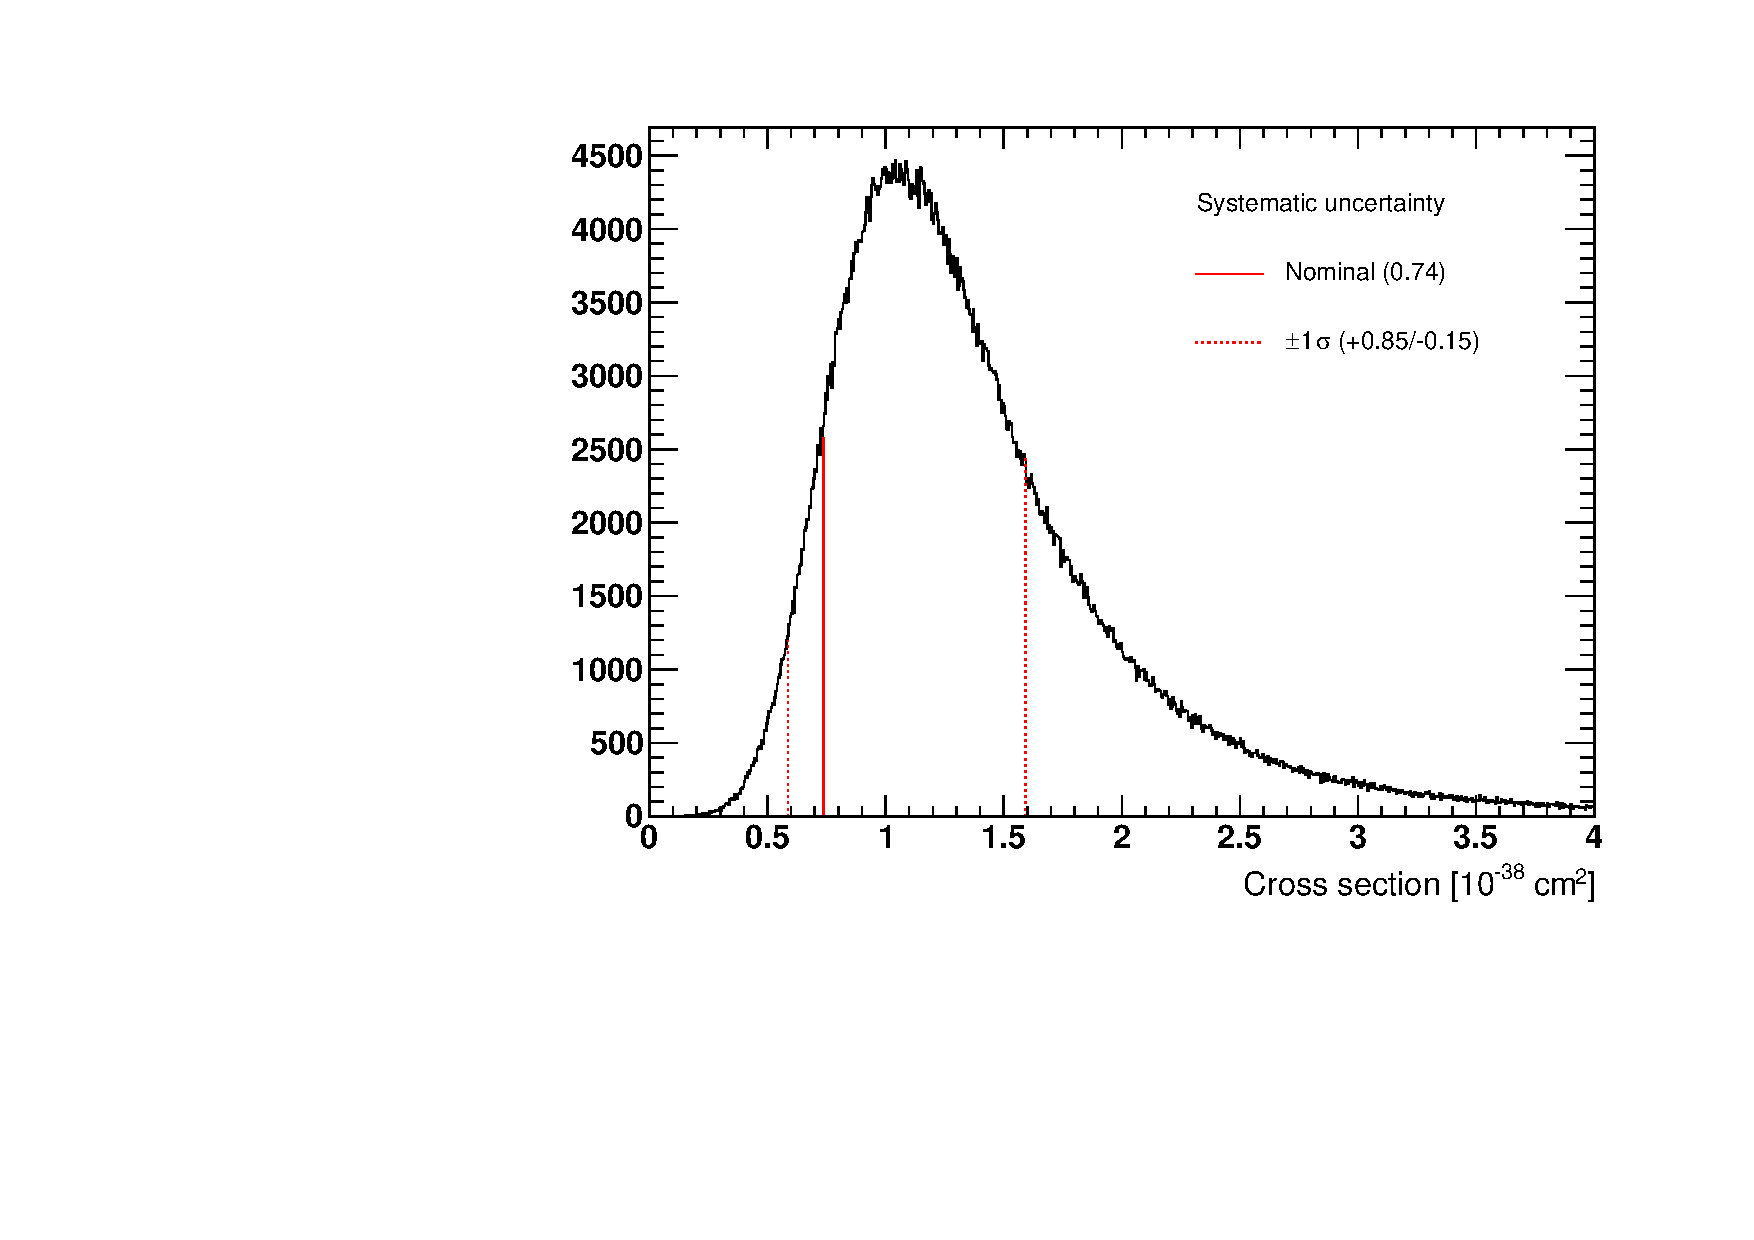
\includegraphics[width=12cm]{PDF/ToyMC/ToyMC}
	\caption[Result of the toy-MC]{
	Result of the toy-MC.
	The 1$\sigma$ confidence level region becomes $[0.59, 1.59] \times 10^{-38}\,{\rm cm}^{2}/{\rm oxygen}$.
	Due to the secondary interaction uncertainty, the peak position is shifted right from the nominal value ($0.74 \times 10^{-38}\,{\rm cm}^{2}/{\rm oxygen}$).
	}\label{ToyMC}
\end{figure}

\begin{figure}[p]
	\centering
	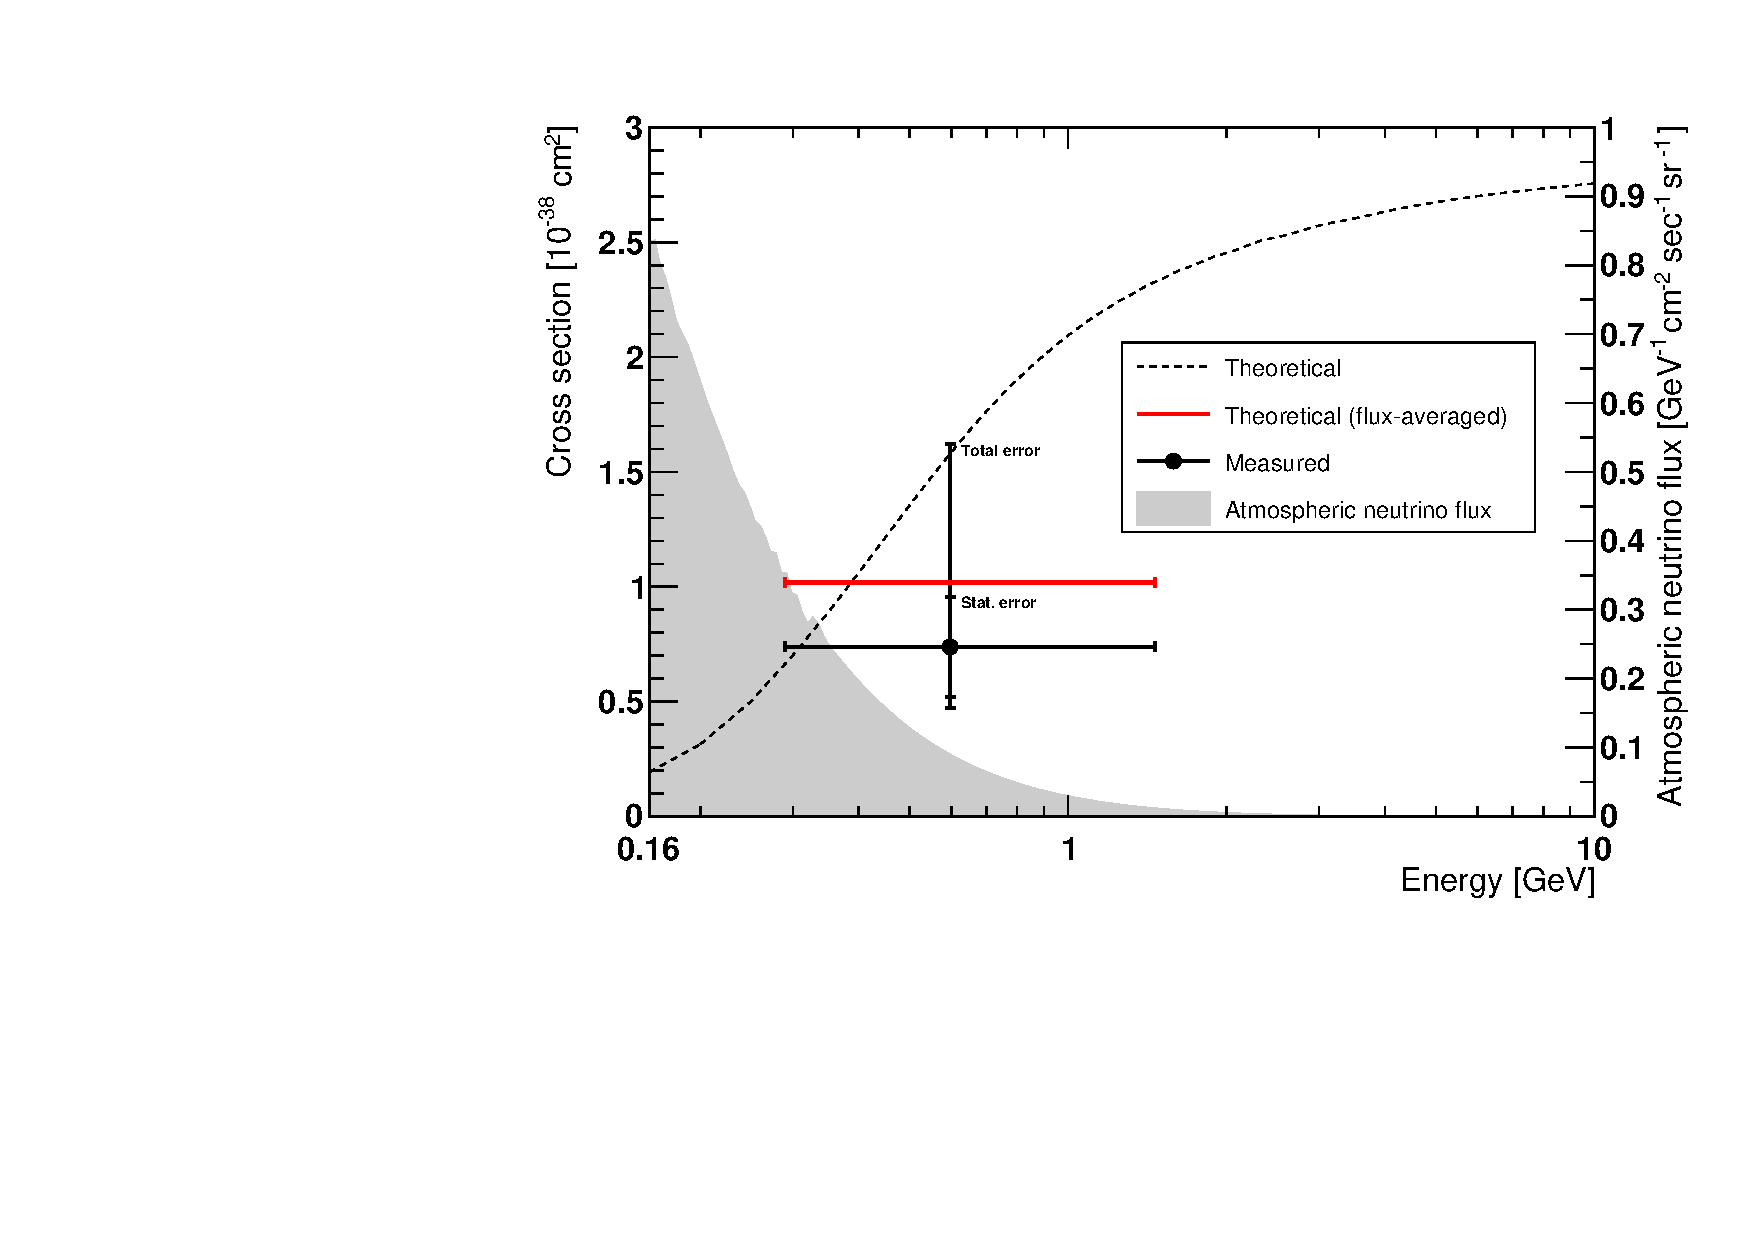
\includegraphics[width=12cm]{PDF/CrossSection/Logx_Figure09}
	\caption[The measured neutrino-oxygen NCQE cross section, the theoretical neutrino-oxygen NCQE cross section, and the atmospheric neutrino flux predicted using the HKKM11 model]{
	The measured neutrino-oxygen NCQE cross section, the theoretical neutrino-oxygen NCQE cross section~\cite{2012Ankowski}, and the atmospheric neutrino flux predicted using the HKKM11 model~\cite{2011Honda}.
	Vertical bars show the statistical uncertainty (short bar) and the total uncertainty (long bar).
	Horizontal bars show the 1$\sigma$ from the mean (0.60~GeV) of the theoretical NCQE cross section multiplied by the atmospheric neutrino flux.
	}\label{Logx_Figure09}
\end{figure}

\begin{figure}[p]
	\centering
	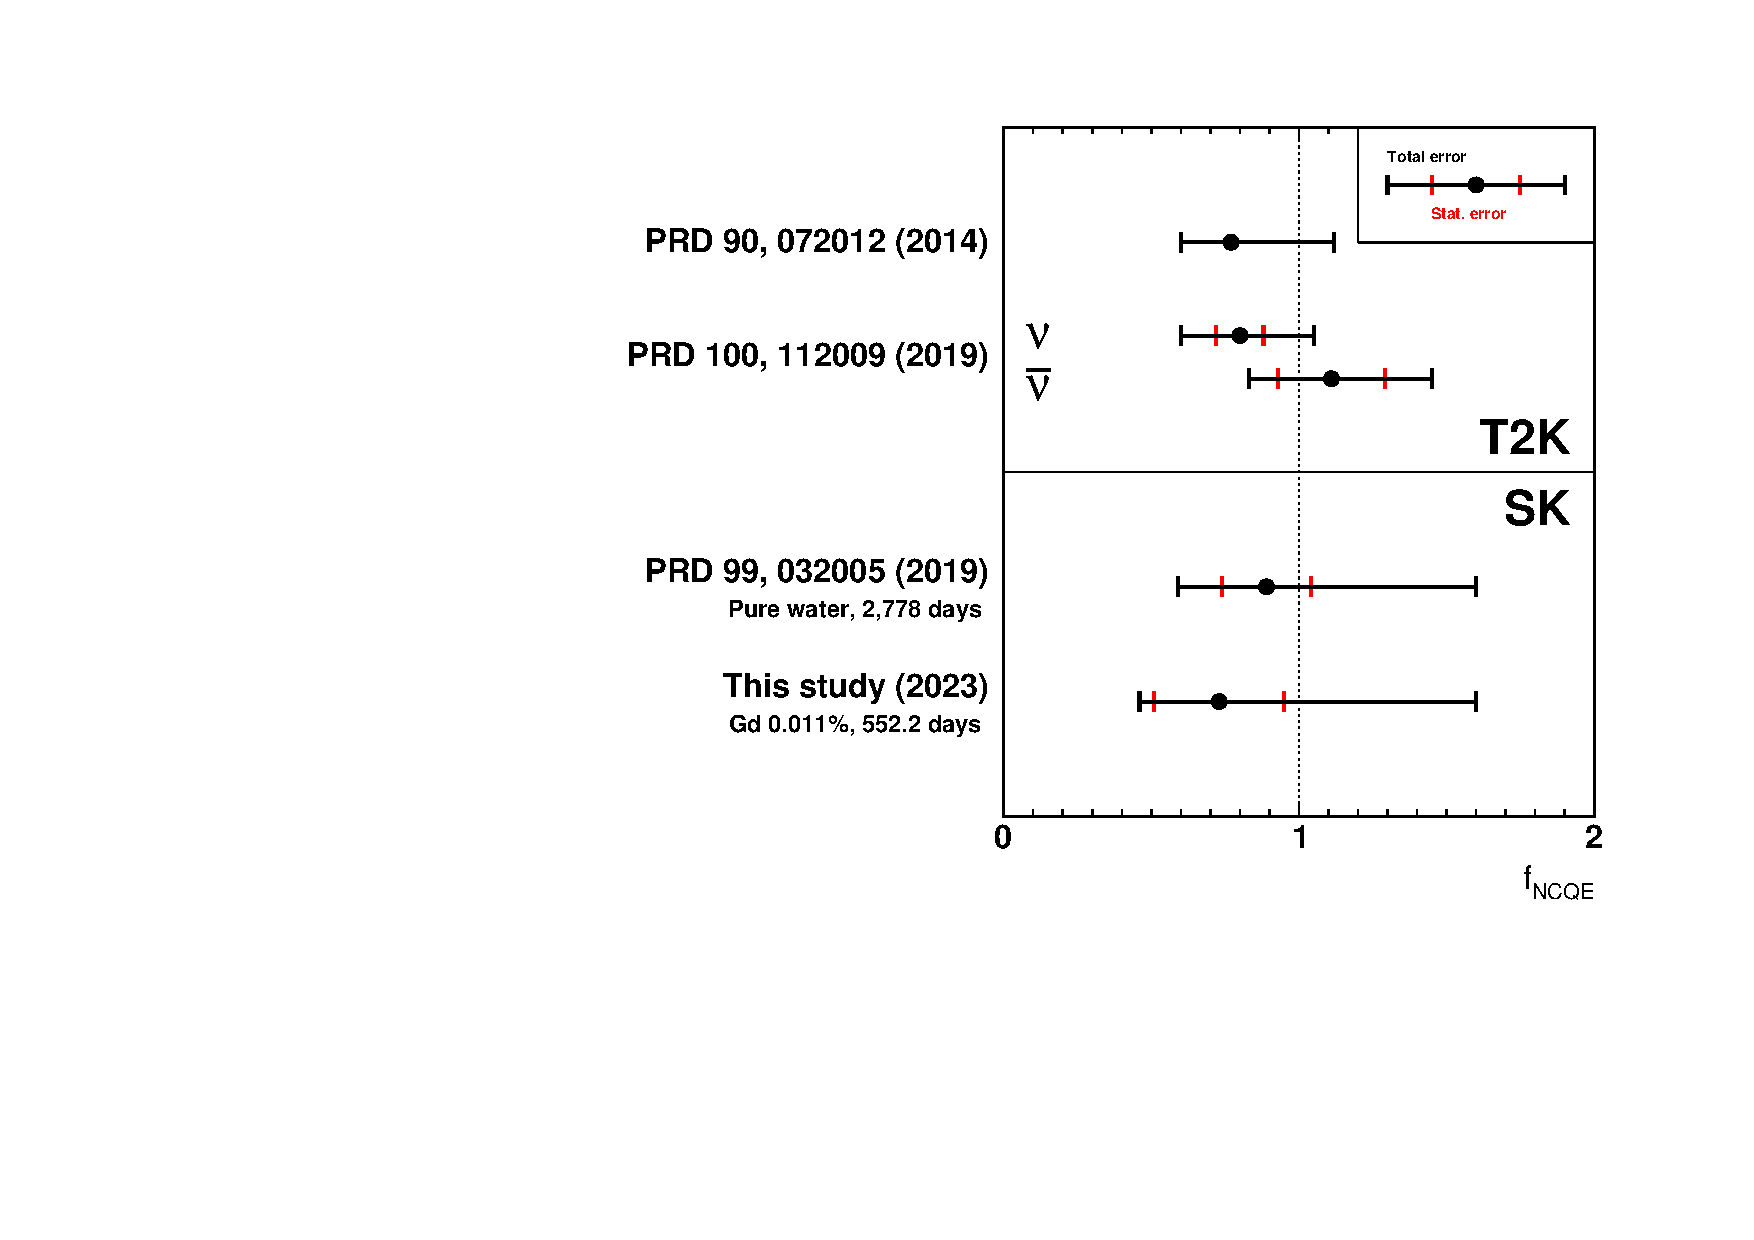
\includegraphics[width=12cm]{PDF/PreviousStudy/PreviousStudy}
	\caption[Comparison of $f_{\rm NCQE}$ with previous measurements in SK and T2K]{
	Comparison of $f_{\rm NCQE}$ (see Equation~(\ref{Eq_f_NCQE})) with previous measurements in SK and T2K~\cite{2014Abe,2019Abe,2019Linyan}.
	Horizontal bars show the statistical uncertainty (short bar) and the total uncertainty (long bar).
	}\label{PreviousStudy}
\end{figure}

\begin{figure}[p]
	\centering
	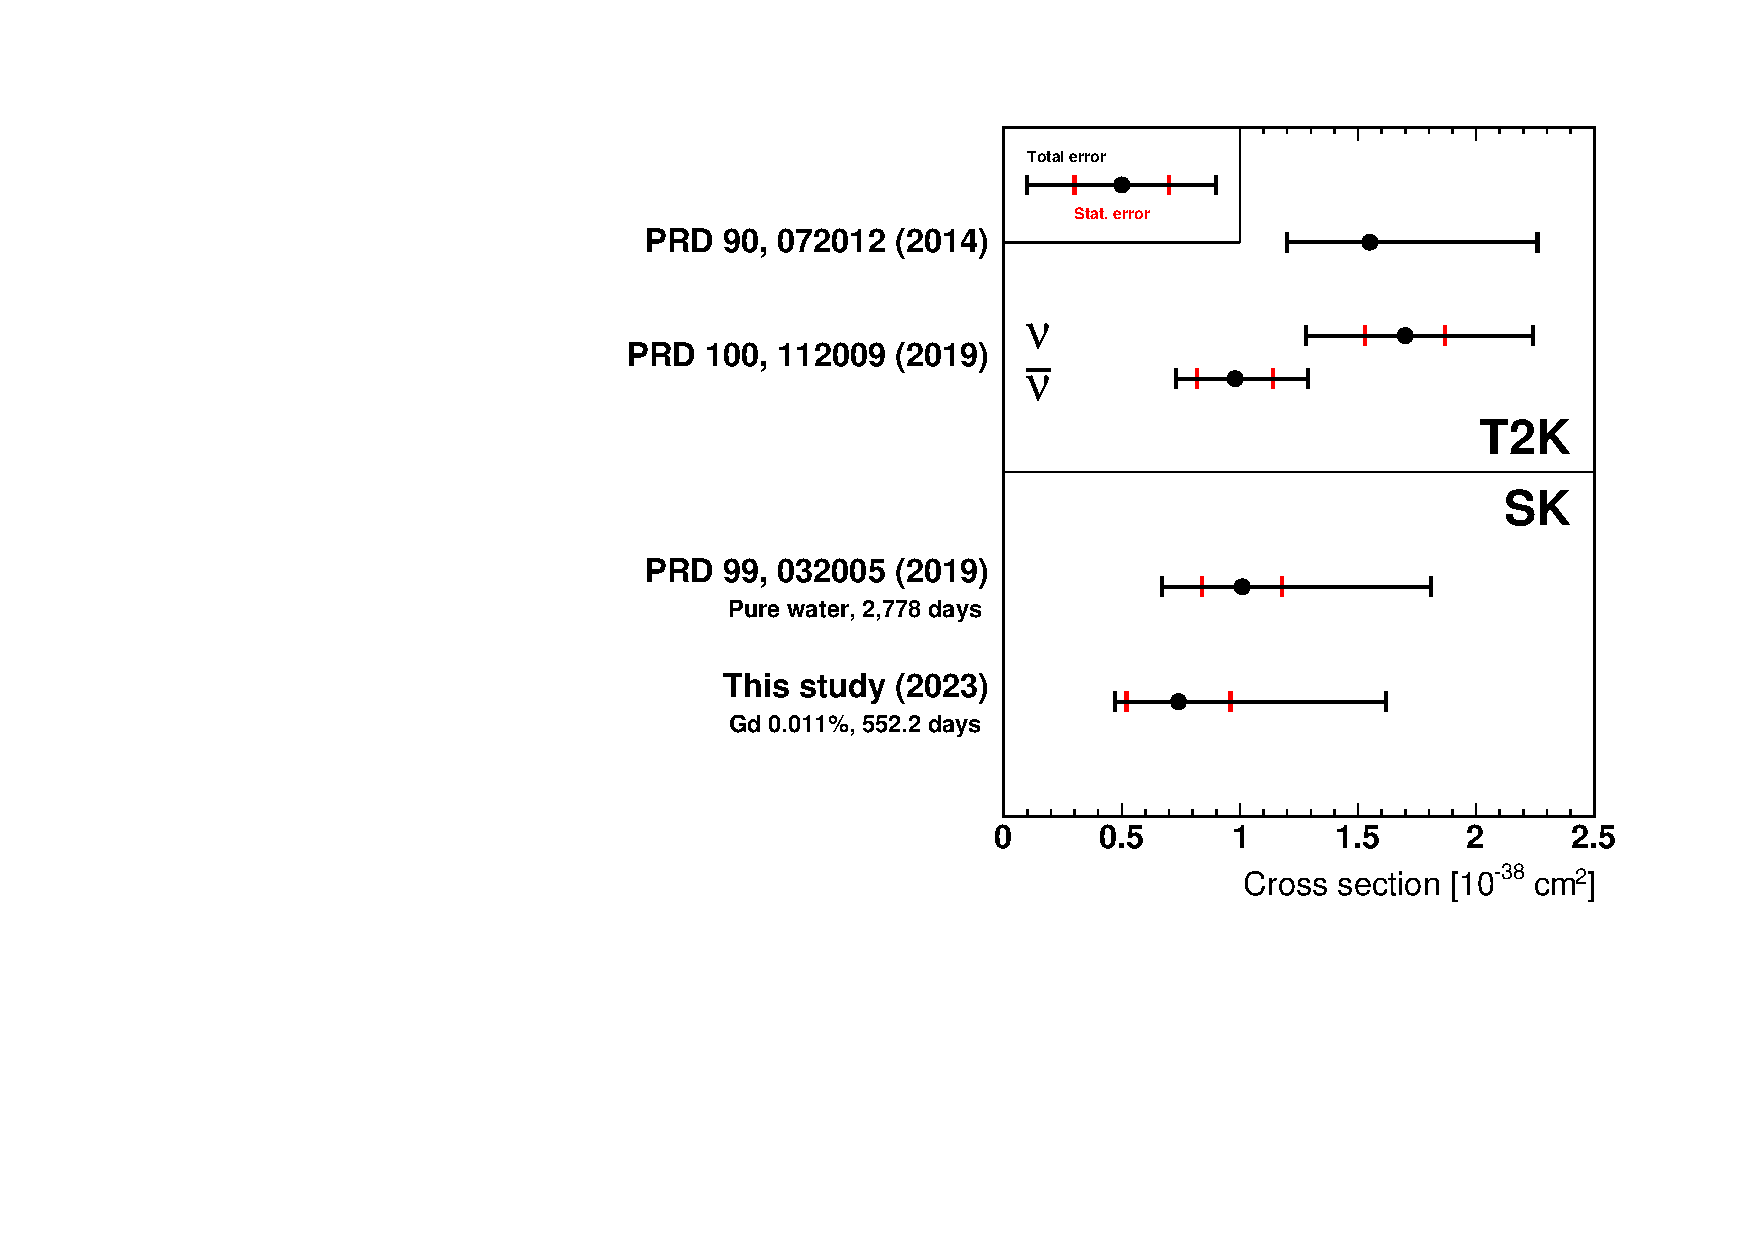
\includegraphics[width=12cm]{PDF/PreviousStudy/PreviousStudy_02}
	\caption[Comparison of the measured neutrino-oxygen NCQE cross section with previous measurements in SK and T2K]{
	Comparison of the measured neutrino-oxygen NCQE cross section with previous measurements in SK and T2K~\cite{2014Abe,2019Abe,2019Linyan}.
	Horizontal bars show the statistical uncertainty (short bar) and the total uncertainty (long bar).
	}\label{PreviousStudy_02}
\end{figure}





\newpage

